











\begin{figure*}[]
\centering
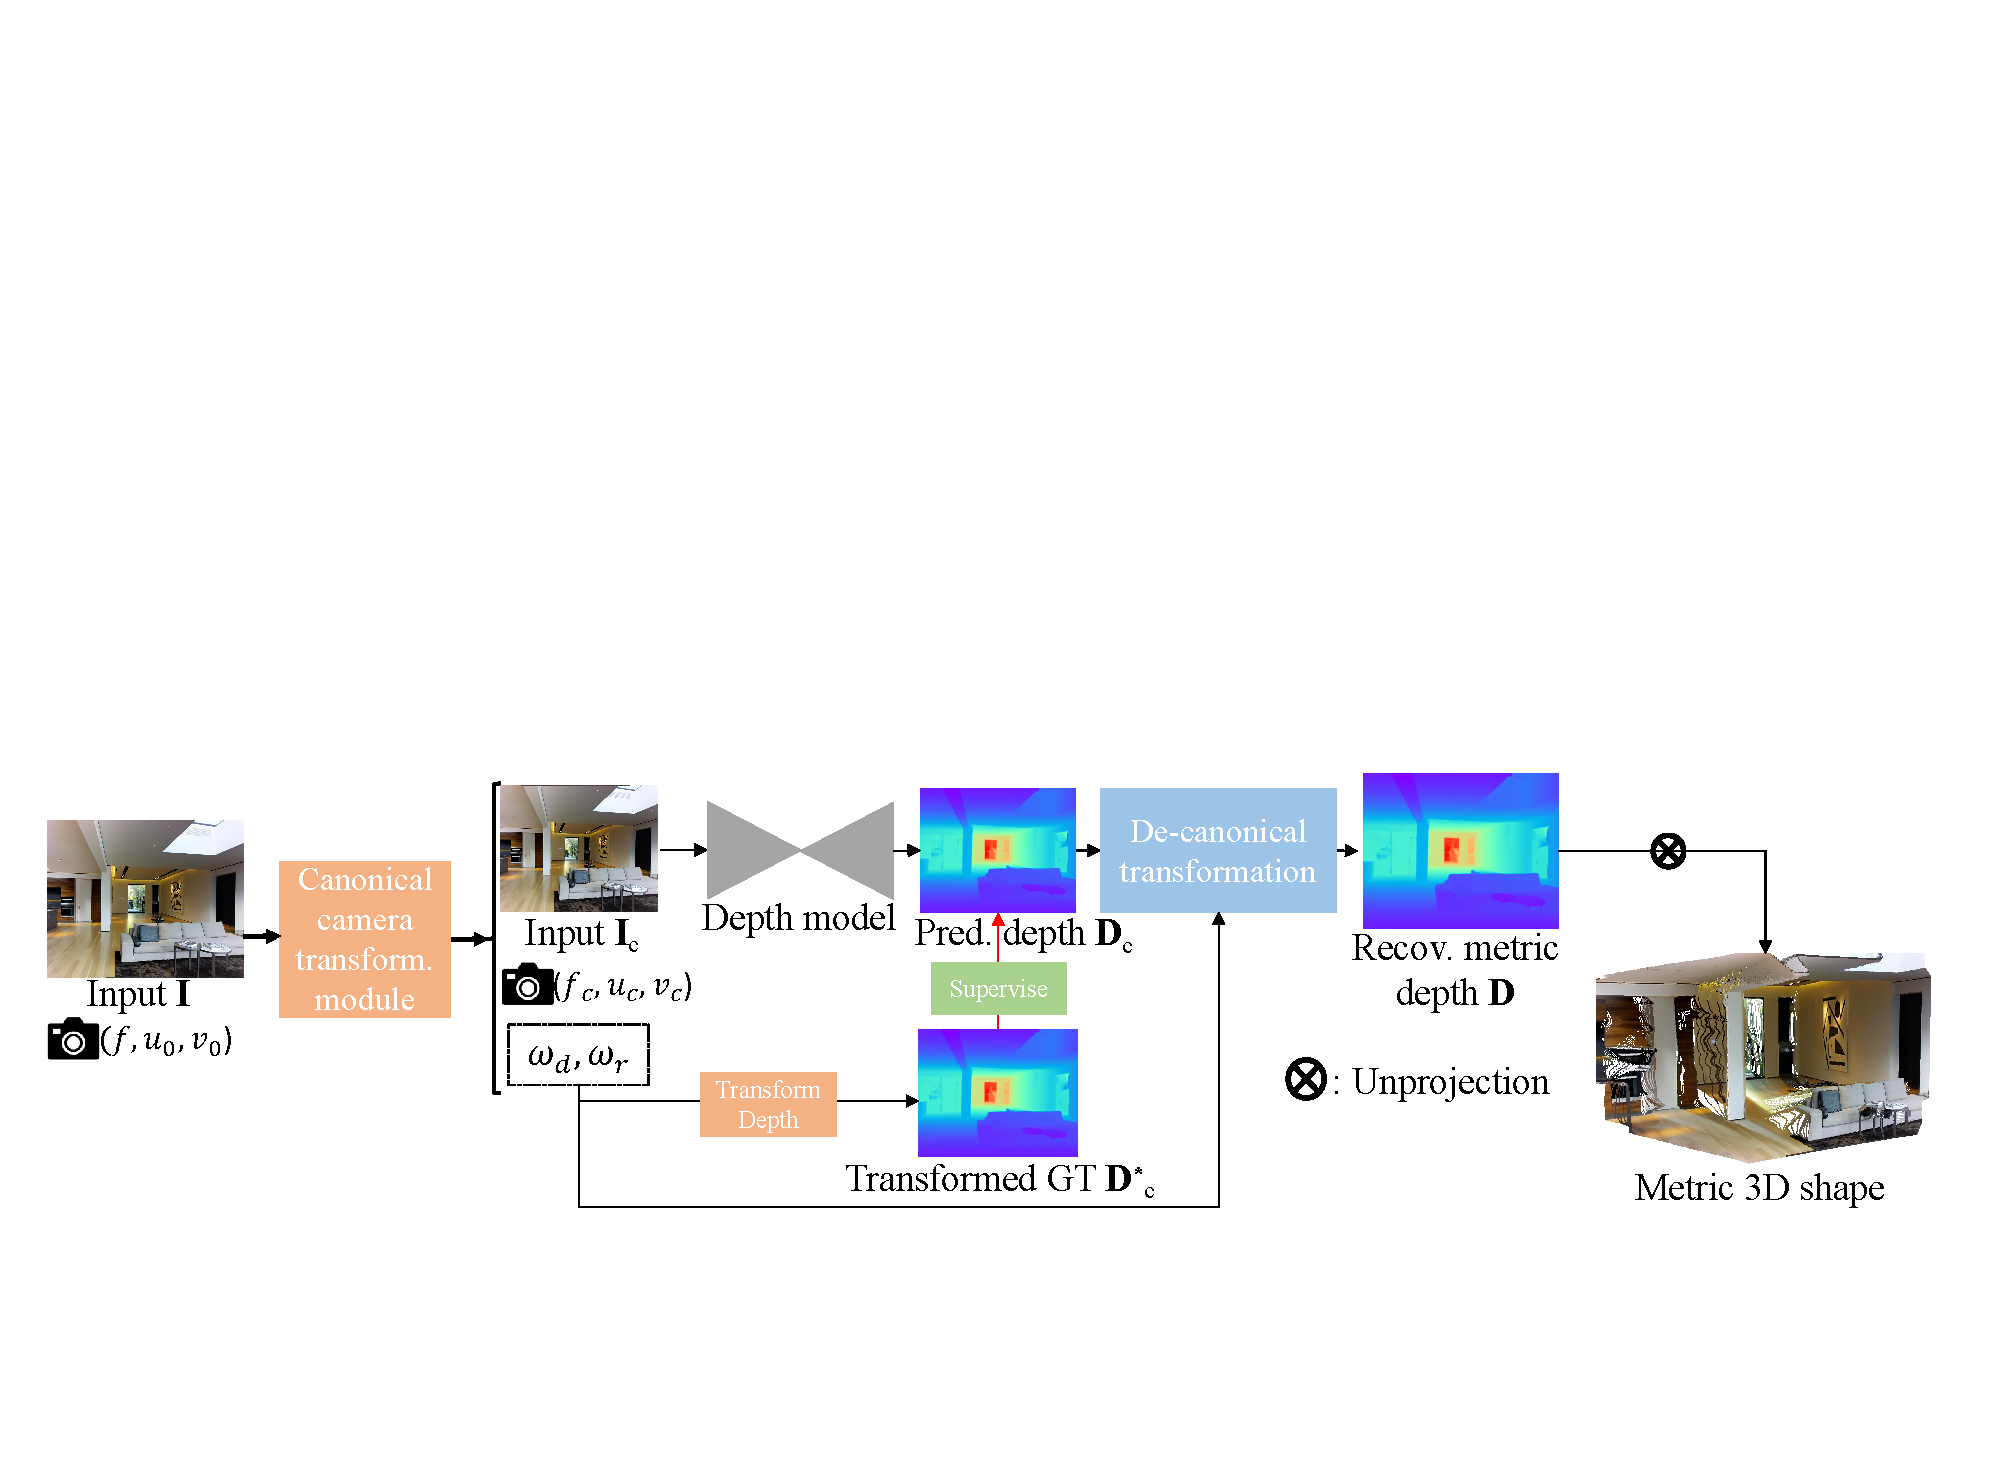
\includegraphics[width=0.99\textwidth]{./files/pipeline3}
\vspace{-1 em}
\caption{\textbf{Pipeline.} 
Given an input image $I$, we first transform it to the canonical space using CSTM. The transformed image $I_c$ is fed into a standard depth estimation model to produce the predicted metric depth $D_c$ in the canonical space. During training, $D_c$ is supervised by a GT depth $D^*_c$ which is also transformed into the canonical space. In inference, after producing the metric depth $D_c$ in the canonical space, we perform a de-canonical transformation to convert it back to the space of the original input $I$. The canonical space transformation and de-canonical transformation are executed using camera intrinsics.}
\label{fig: pipeline}
\vspace{-1em}
\end{figure*}

\noindent\textbf{Preliminaries.}
We consider the pin-hole camera model with intrinsic parameters are:
[[$\nicefrac{\hat{f}}{\delta}, 0, u_{0}$], [$0,  \nicefrac{\hat{f}}{\delta},  v_{0}$], [$0, 0,  1$]],
where $\hat{f}$ is the 
focal length (in micrometers), $\delta$ is the pixel size
(in micrometers), and
$(u_{0}, v_{0})$ is the principle center. $f = \nicefrac{\hat{f}}{\delta}$ is the pixel-represented focal length used in vision algorithms.








\subsection{Metric Ambiguity Analysis}\label{sec:ambiguity}

Fig.~\ref{fig: inspiration} presents an example of photos taken by different cameras and at 
different distances. Only from the image's appearance, 
one may think 
the last two photos are taken at %
a 
similar location by the same camera. %
In fact, due to different focal lengths, 
these %
are captured at different locations.
Thus, 
camera %
intrinsic parameters are 
critically 
important for the metric estimation from a single image, as otherwise, the problem is \textit{ill posed}. 
To avoid such metric ambiguity, recent %
methods, such as MiDaS~\cite{Ranftl2020} and LeReS~\cite{leres}, decouple the metric from the supervision and %
compromise learning the affine-invariant depth.



\begin{figure}[!bt]
\centering
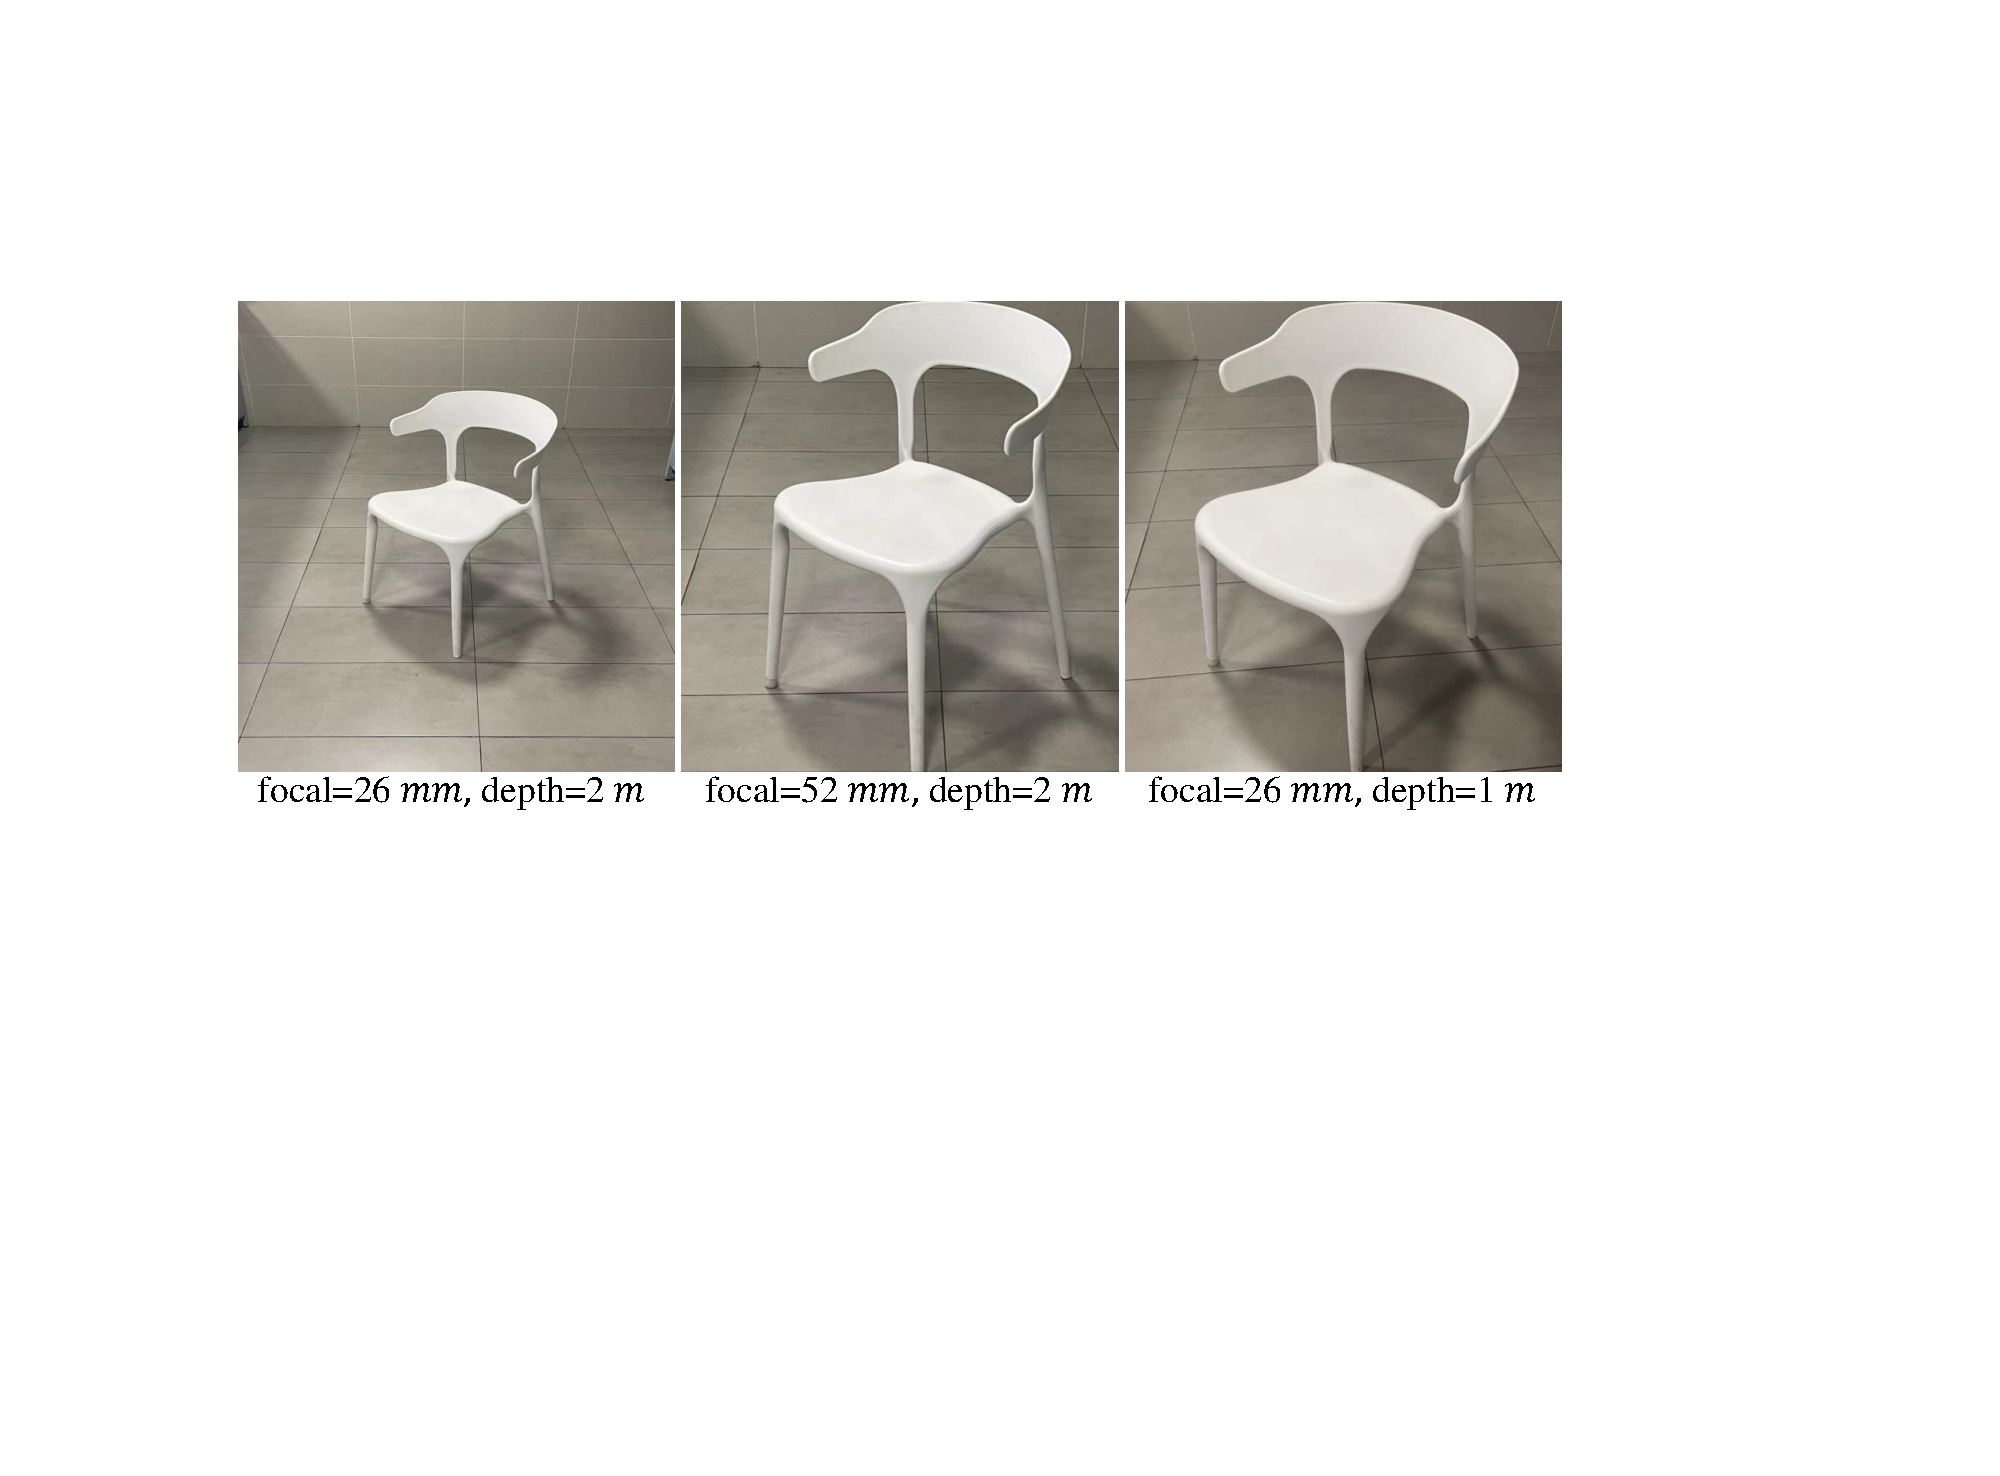
\includegraphics[width=0.47\textwidth]{./files/inspiration}
\vspace{-0.5 em}
\caption{\textbf{Photos of a chair captured at different distances with different cameras}. The first two photos are captured at the same distance but with different cameras, 
while the last one is taken at a closer distance with the same camera as the first one.}
\label{fig: inspiration}
\vspace{-1.5em}
\end{figure}

Fig.~\ref{fig: pinhole camera} (A) shows a simple pin-hole perspective projection. Object $A$ locating at $d_{a}$ is projected to $A'$. 
Based on the principle of similarity, we %
have the equation:
\begin{equation}
\vspace{-1em}
    d_{a} = \hat{S} \Bigl[\frac{\hat{f}}{\hat{S'}}\Bigr]= \hat{S}\cdot \alpha
\label{eq: similarity}
\end{equation}
where $\hat{S}$ and $\hat{S'}$ are the real and \textit{imaging} size respectively. $\hat{\cdot}$ denotes variables are in the physical metric (\textit{e.g.}, millimeter). To %
recover 
$d_{a}$ from a single image, focal length, imaging size of the object, and real-world object size %
must be available. 
Estimating the focal length 
from a single image is a %
challenging 
and ill-posed problem. Although several methods~\cite{leres, hold2018perceptual} have explored,
the accuracy 
is still far from being satisfactory. 
Here, we simplify the problem by assuming 
the focal length of a training/test image is available. 
In contrast, understanding the imaging size is much easier for a neural network. To obtain the real-world object size, a neural network %
needs to 
understand the semantic scene layout and the object, at which a neural network excels. 
We %
define 
$\alpha = \nicefrac{\hat{f}}{\hat{S'}} $, so $d_{a}$ is proportional to $\alpha$. 
\begin{figure}[!b]
\vspace{-2em}
\centering
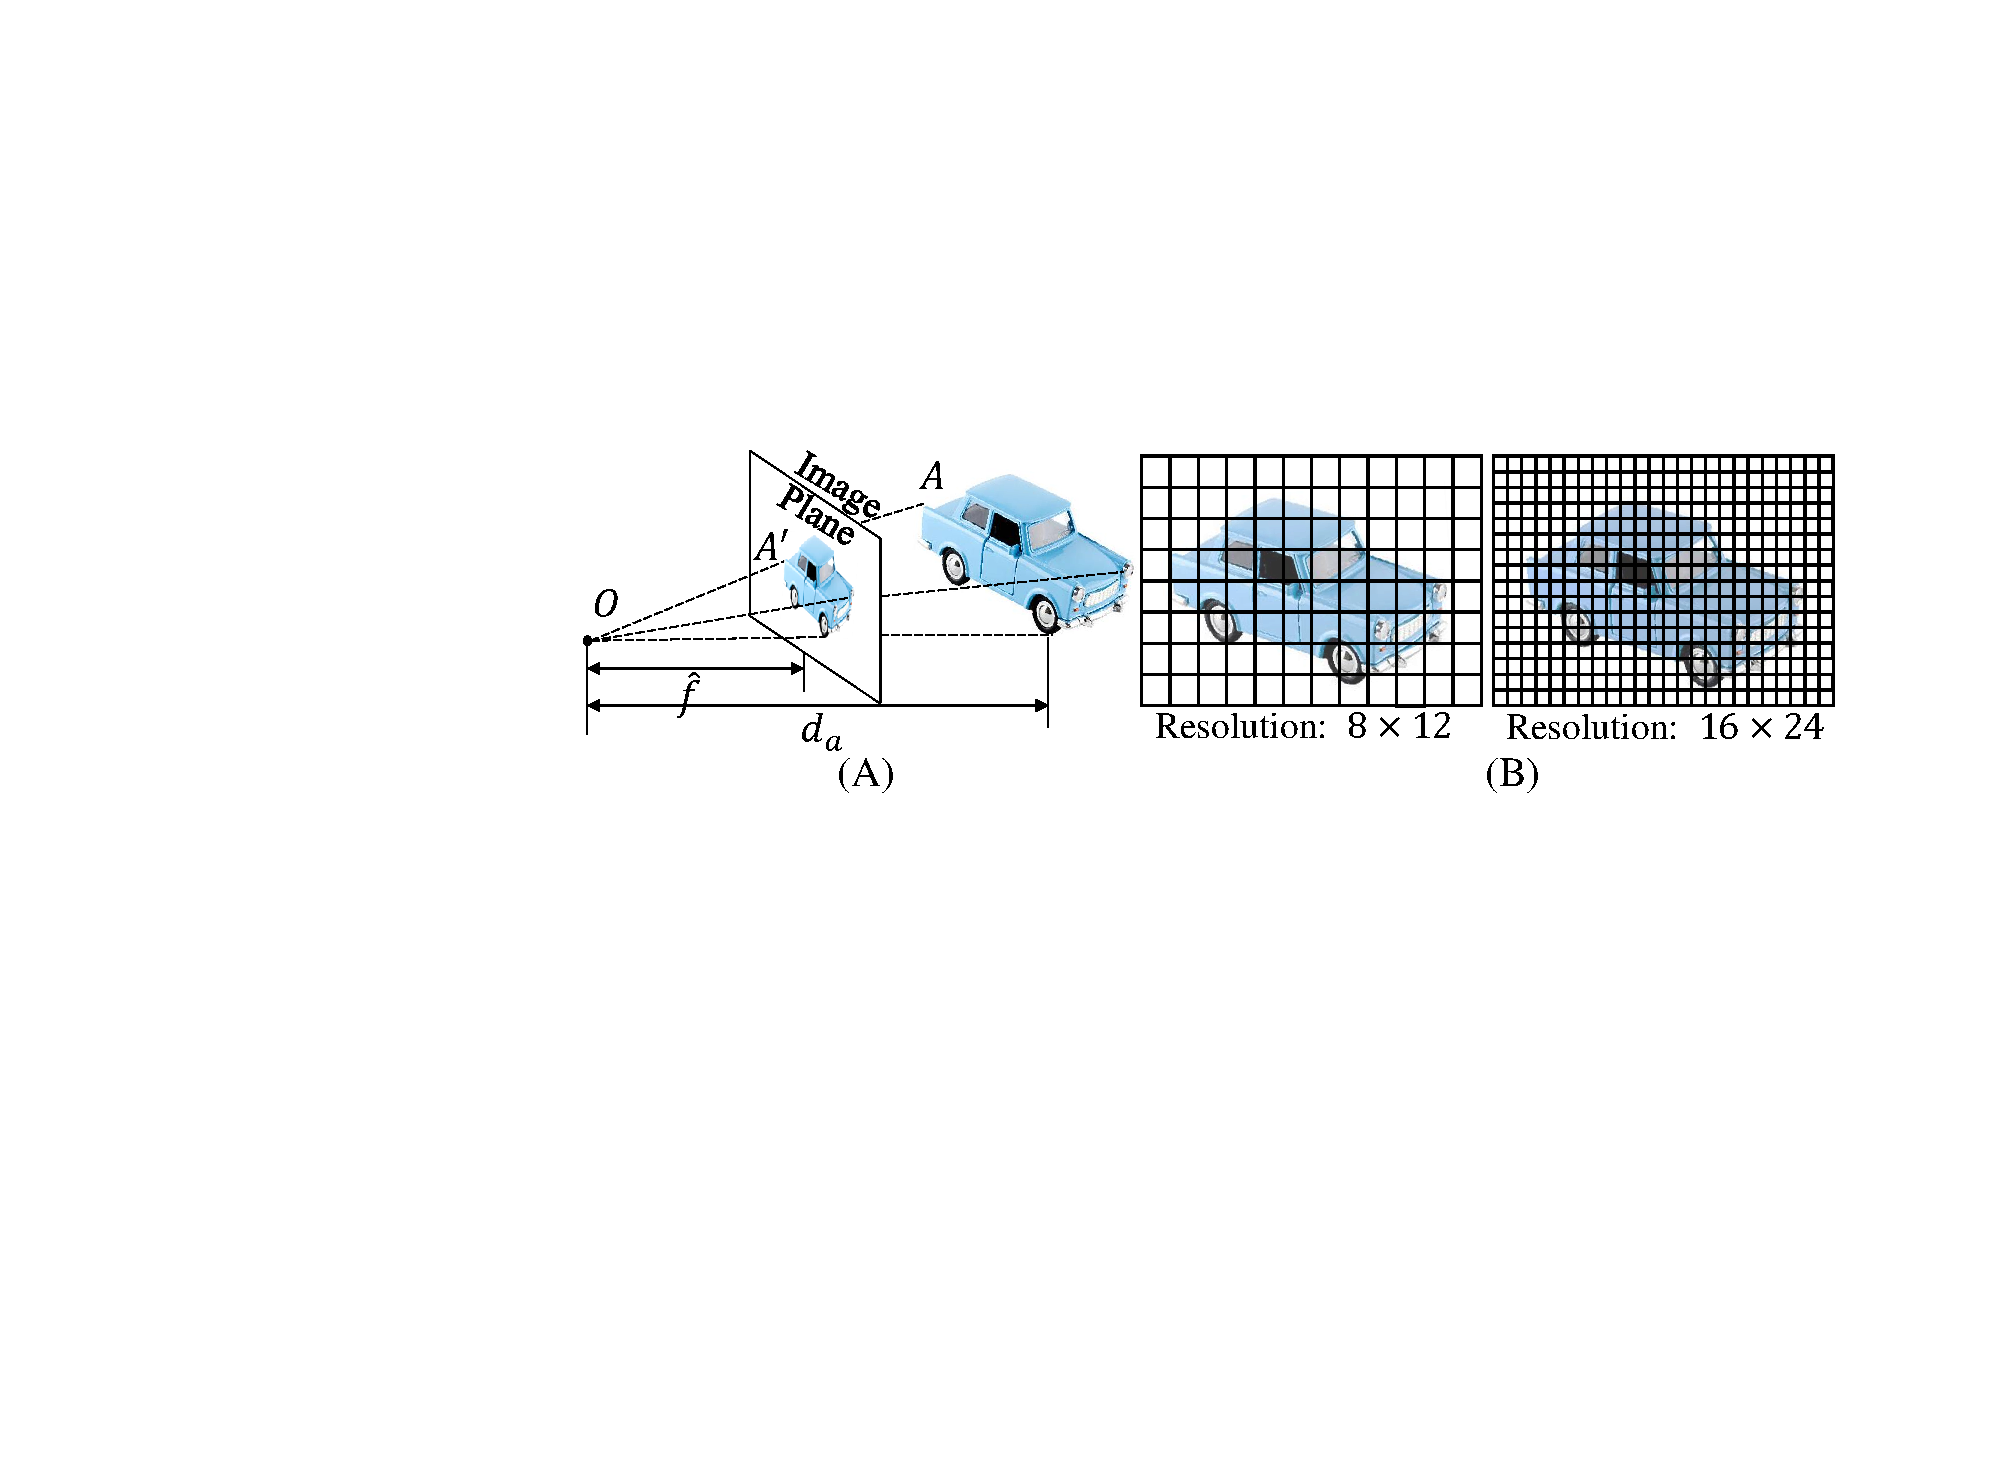
\includegraphics[width=0.5\textwidth]{./files/pinhole_difference_distances}
\caption{\textbf{Pinhole camera model}. (A) Object $A$ at the distance $d_{a}$ is projected to the image plane. (B) Using two cameras to capture the car. The left one has a larger pixel size. Although the projected imaging sizes are the same, the pixel-represented images (resolution) are different.}
\label{fig: pinhole camera}
\vspace{-0.5em}
\end{figure}

We make the following observations regarding sensor size, pixel size, and focal length.


\noindent\textbf{O1: Sensor size and pixel size do not affect the metric depth estimation.} 
Based on the perspective projection (Fig.~\ref{fig: pinhole camera} (A)), the sensor size only affects the field of view (FOV) and is irrelevant to $\alpha$, thus does not affect the metric depth estimation. 
For the pixel size, %
we assume two cameras with different pixel sizes ($\delta_{1} = 2\delta_{2}$) but the same focal length $\hat{f}$ to capture the same object locating at $d_{a}$. %
Fig.~\ref{fig: pinhole camera} (B) shows their captured photos.
According to the preliminaries, %
the pixel-represented focal length $f_{1} = \frac{1}{2} f_{2}$. 
As the second camera has a smaller pixel size, although in the same projected imaging size $\hat{S'}$, the pixel-represented image resolution is $S'_{1} = \frac{1}{2} S'_{2}$. According to Eq.~\eqref{eq: similarity}, $\frac{\hat{f}}{\delta_{1}\cdot S'_{1}} = \frac{\hat{f}}{\delta_{2}\cdot S'_{2} }$, i.e. $\alpha_1 = \alpha_2$, so $d_{1} = d_{2}$. Therefore, different camera sensors %
would 
not affect the metric depth estimation.


\noindent\textbf{O2: The focal length is vital for %
metric depth estimation}. Fig.~\ref{fig: inspiration} shows the metric ambiguity issue caused by the unknown focal length. 
Fig.~\ref{fig: confusion} %
illustrates 
this. If two cameras ($\hat{f}_{1} = 2\hat{f}_{2}$) are at distances $d_{1} = 2d_{2}$, the imaging sizes on cameras are the same. Thus, only from the appearance, %
the network will be confused when supervised with different labels.
Based on this observation, we propose a canonical camera transformation method to solve the supervision and image appearance conflicts.

\begin{figure}[!bt]
\centering
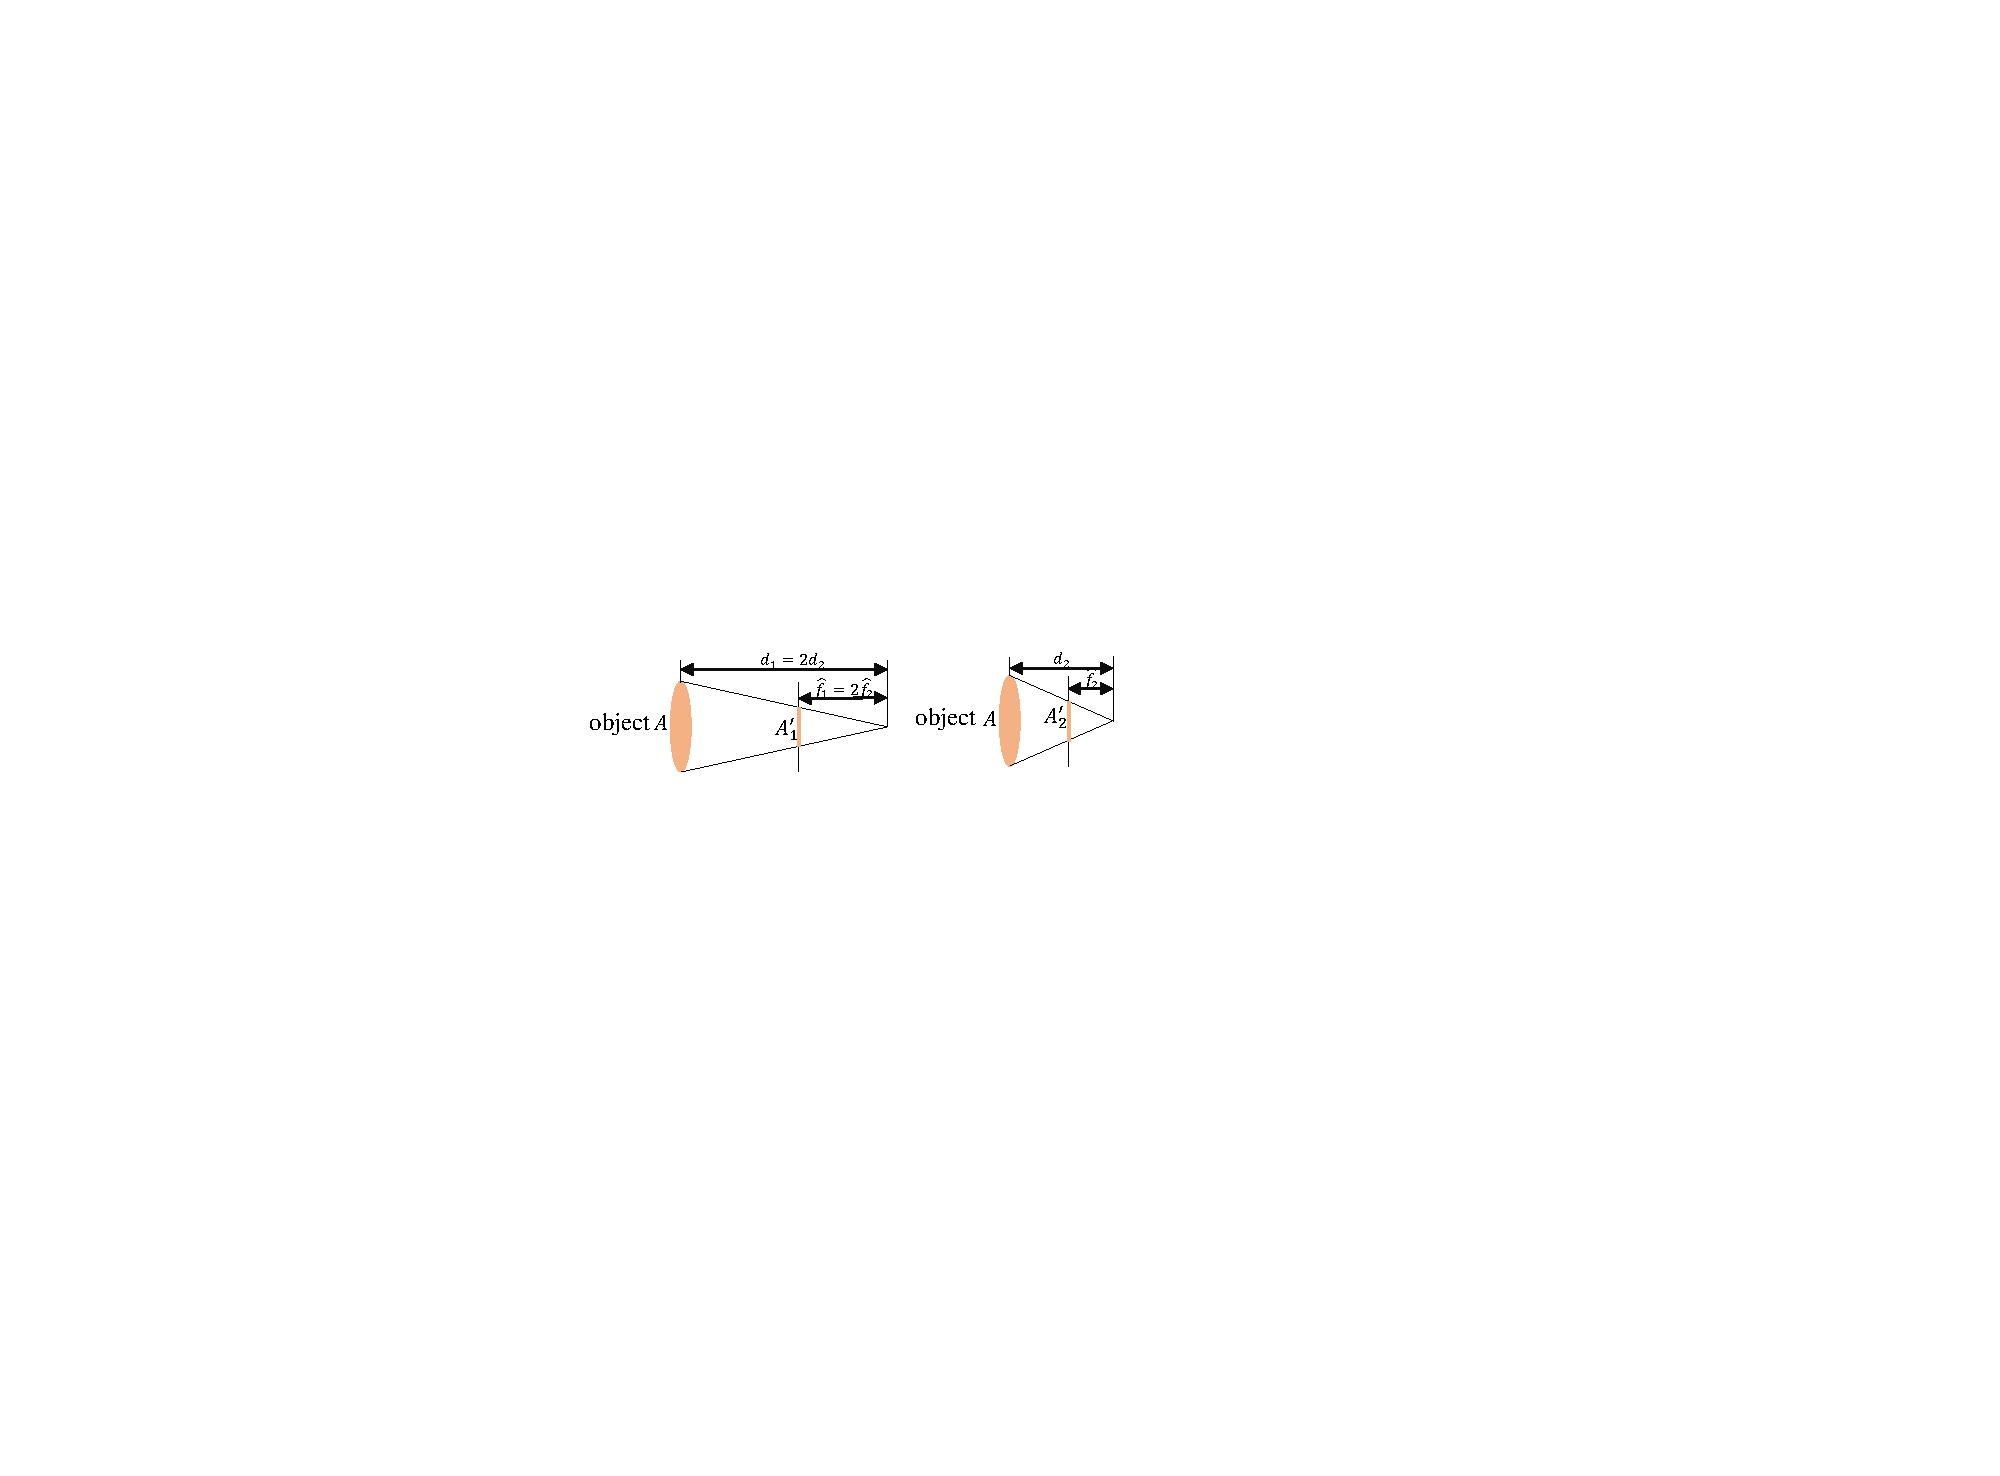
\includegraphics[width=0.48\textwidth]{./files/confusion}
\caption{\textbf{Illustration of two cameras with different focal length} at different distance. As $f_1=2f_2$ and $d_1=2d_2$, 
$A$ is projected 
to two image planes with the same imaging size (i.e. $A^{'}_1 = A^{'}_2$).
}
\label{fig: confusion}
\vspace{-2em}
\end{figure}




\subsection{Canonical Camera Transformation}
The core idea is to set up a canonical camera space ($(f_{x}^{c}, f_{y}^{c})$, $f_{x}^{c}=f_{y}^{c}=f^{c}$ in experiments) and transform all training data to this space. 
Consequently, all data can roughly be regarded as captured by the canonical camera.
We propose two transformation methods, i.e. either transforming the input image ($\mathbf{I}\in\mathbb{R}^{H \times W \times 3}$) or the ground-truth (GT) label ($\mathbf{D}\in\mathbb{R}^{H \times W}$). The original intrinsics are $\{f, u_{0}, v_{0}\}$.

\noindent\textbf{Method1: transforming depth labels (CSTM\_label).}
Fig.~\ref{fig: inspiration}'s ambiguity is for depths. 
Thus our first method directly transforms the ground-truth depth labels to solve this problem.  Specifically, we scale the ground-truth depth ($\mathbf{D}^{*}$) with the ratio $\omega_d = \frac{f^{c}}{f}$ in training, \textit{i.e.},  $\mathbf{D}^{*}_{c} = \omega_d \mathbf{D}^{*}$. The original camera model is transformed to $\{f^{c}, u_{0}, v_{0}\}$. In inference, the predicted depth ($\mathbf{D}_{c}$) is in the canonical space and needs to perform a de-canonical transformation to recover the metric information, \textit{i.e.}, $\mathbf{D} = \frac{1}{\omega_d}\mathbf{D}_{c}$. Note the input $\mathbf{I}$ does not perform any transformation, \textit{i.e.},  $\mathbf{I}_c = \mathbf{I}$.

\noindent\textbf{Method2: transforming input images (CSTM\_image).}
From another view, the ambiguity is caused by the similar image appearance. Thus this method is to transform the input image to simulate the canonical camera imaging effect.
Specifically, the image $\mathbf{I}$ is resized with the ratio $\omega_r=\frac{f^{c}}{f}$, \textit{i.e.},
$\mathbf{I}_{c} = \mathcal{T}(\mathbf{I}, \omega_r)$, where $\mathcal{T}(\cdot)$ denotes image resize. The optical center is resized, thus the canonical camera model is $\{f^{c}, \omega_r u_{0}, \omega_r v_{0}\}$. The ground-truth labels are resized without any scaling, \textit{i.e.}, 
$\mathbf{D}^{*}_{c} = \mathcal{T}(\mathbf{D}^*, \omega_r)$. In inference, the de-canonical transformation is to resize the prediction to the original size without scaling, \textit{i.e.}, $\mathbf{D} = \mathcal{T}(\mathbf{D}_{c}, \frac{1}{\omega_r})$.

Fig.~\ref{fig: pipeline} shows the pipeline. After performing either transformation, we randomly crop a patch for training. %
The cropping only adjusts the FOV and the optical center, %
thus not causing any metric ambiguity issues. In the labels transformation method $\omega_r = 1$ and $\omega_d=\frac{f^c}{f}$, while $\omega_d = 1$ and $\omega_r=\frac{f^c}{f}$ in the images transformation method. The training objective is as follows:
\begin{equation}
    \min_{\theta}\left | \mathcal{N}_{d}(\mathbf{I}_{c}, \theta) - \mathbf{D}^{*}_{c} \right| 
\label{eq: robust metric depth}
\vspace{-0.5 em}
\end{equation}
where 
$\theta$ is the network's ($\mathcal{N}_{d}(\cdot)$) parameters, $\mathbf{D}^{*}_{c}$ and $\mathbf{I}_{c}$ are transformed ground-truth depth labels and images.




Mix-data training is an effective way to boost generalization. 
We collect $11$ datasets for training, see 
the supplementary materials for details. In the mixed data, over 10K different cameras are included. %
All collected training data have included paired camera intrinsic parameters, which are %
used in our canonical transformation module. 


\noindent\textbf{Supervision.} To further boost the performance, we propose a random proposal normalization loss (RPNL). The scale-shift invariant loss~\cite{Ranftl2020, leres} is widely applied for the affine-invariant depth estimation, which decouples the depth scale to emphasize the single image distribution. However, such normalization based on the whole image inevitably squeezes the fine-grained depth difference, particularly in close regions. Inspired by this, we propose to randomly crop several patches ($p_{i(i=0,...,M)} \in \mathbb{R}^{h_i \times w_i}$) from the ground truth $\mathbf{D}^{*}_c$ and the predicted depth $\mathbf{D}_c$. Then we employ the median absolute deviation normalization~\cite{singh2019investigating} for paired patches. By normalizing the local statistics, we can enhance local contrast. The loss function is as follows:
\begin{eqnarray}\nonumber
    L_{\RPNL} = \frac{1}{MN} \sum_{p_i}^{M}\sum_{j}^{N} \lvert \frac{d^{*}_{p_i, j} - \mu(d^{*}_{p_i, j})}{\frac{1}{N}\sum_{j}^{N} \left |d^{*}_{p_i, j} - \mu(d^{*}_{p_i, j}) \right |} - \\
    \frac{d_{p_i, j} - \mu(d_{p_i, j})}{\frac{1}{N}\sum_{j}^{N} \left | d_{p_i, j} - \mu(d_{p_i, j}) \right |} \rvert
\label{eq: RPNL}
\end{eqnarray}
where $d^*\in \mathbf{D}^*_c$ and $d \in \mathbf{D}_c$ are the ground truth and predicted depth respectively. $\mu(\cdot)$ and is the median of depth. $M$ is the number of proposal crops, which is set to 32. During training, proposals are randomly cropped from the image by 
$0.125$ to $0.5$ of the original size. Furthermore, several other losses are employed, including the scale-invariant logarithmic loss~\cite{eigen2014depth} $L_{silog}$, pair-wise normal regression loss~\cite{leres}$L_{\PWN}$, virtual normal loss~\cite{yin2021virtual} $L_{\VNL}$. Note $L_{silog}$ is a variant of L1 loss.  The overall losses are as follows.
\begin{eqnarray}\nonumber
    L = L_{\PWN} + L_{\VNL} + L_{silog} + L_{\RPNL}.
\label{eq: losses}
\end{eqnarray}
\vspace{-2 em}

